\section{Introduction}
Agriculture is one of the most fundamental resource of food production and also plays a vital role in keeping the economy running of every nation by contributing to the Gross Domestic Production. But there are several issues related to traditional methods of agriculture such as excessive wastage of water during irrigation of field, dependency on non-renewable power source, time, money, human resource etc. Since every activity now a days becoming smart it needs to smartly develop agriculture sector for growth of country. Out project aims at developing a Smart Irrigation System using IoT Technology with an objective of automating the total irrigation system which provide adequate water required by crop by monitoring the moisture of soil and climate condition in order to prevent the wastage of water resource. It will also have many advantages for farmers. The irrigation at remote location from home will become easy and more comfortable. In addition, it will not only protect the farmer from scorching heat and severe cold but also save their time for to and from journey to the field.



\subsection{Deployment Structure}
The objective of this project is to adopt a smart irrigation system to water cultivated fields making use of the local water resources, such as aquifers and reservoirs, in the way of using the water resources as more eco-friendly as possible (e.g., without disrupting aquifers). Thus, we can consider two different locations to takes care: the \textbf{field} and the \textbf{water provisioning site},

For what concern the \textit{water provisioning site}, it is composed of sensors which have the mean of monitoring the water level both of the aquifers and reservoirs. In this way, the system and the user can know where to take water (by default the reservoir). Although, a single device for source may be enough, we decided to deploy multiple water level sensors in the same source in order to avoid errors in the monitoring (e.g., in the case of a single device if it is detected that the reservoir is empty, but it is not, the irrigation system will use the water from the aquifer pointlessly).
All water level sensors will make use of \textit{MQTT} as explained in the "MQTT Network" chapter.


The \textit{field site} is more articulated and will exploit multiple types of sensors and a single type of actuator. The actuator needed is the one capable of providing the water to the plants, which we called "tap actuator". This we be used in conjunction with the other sensors presents in the fields that will monitor the environment, specifically there will be temperature sensors, soil moisture sensors and a rain sensor. 
All these sensors and the tap actuator will exploit \textit{CoAP} as explained in the "CoAP Network" chapter.


\begin{figure}[H]
	\begin{subfigure}{\textwidth}
	\centering
		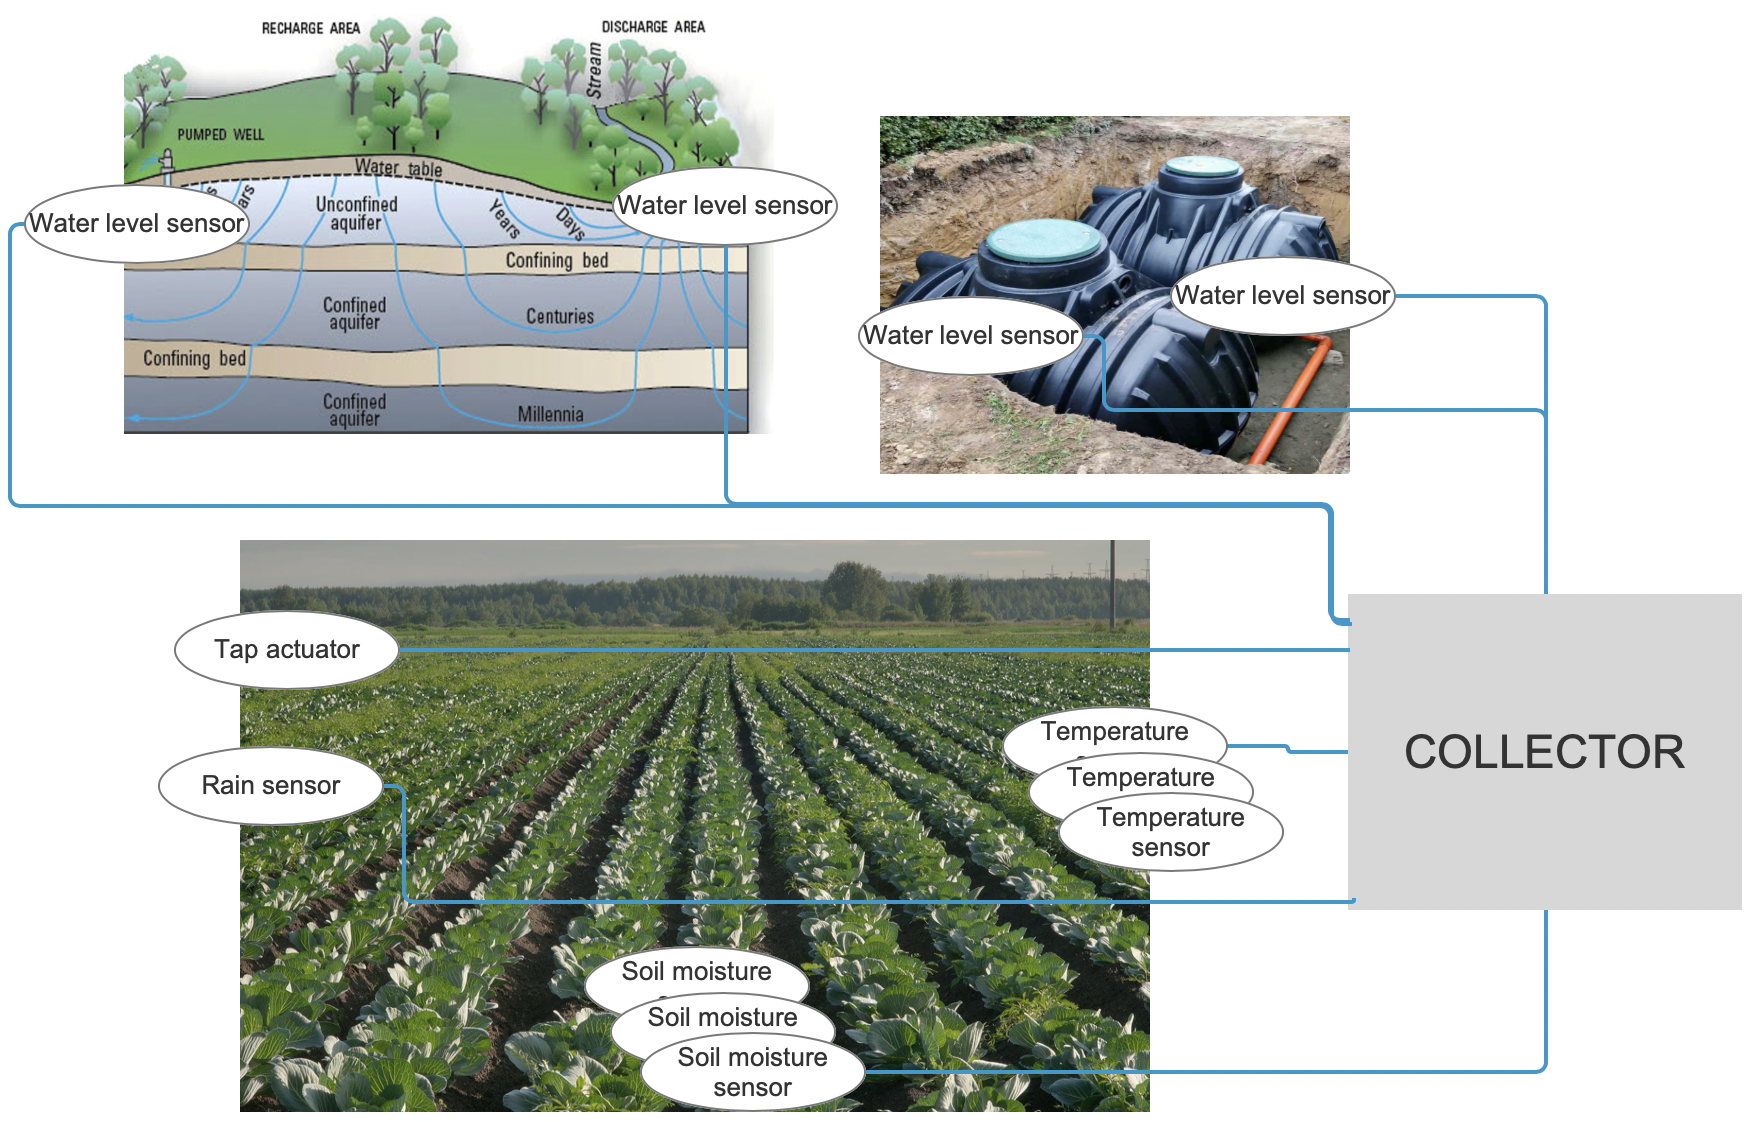
\includegraphics[width=0.66\linewidth]{img/deployment.png} 
	\end{subfigure}
\end{figure}